\section{Structures et matériaux}

%https://fr.wikipedia.org/wiki/Configuration_d%27aile
%https://fr.wikipedia.org/wiki/Profil_(a%C3%A9rodynamique)
%en.wikipedia.org/wiki/Airfoil
%https://fr.wikipedia.org/wiki/Portance_(a%C3%A9rodynamique)
%https://fr.wikipedia.org/wiki/Phare_et_feu_(a%C3%A9ronautique)#:~:text=Ils%20sont%20g%C3%A9n%C3%A9ralement%20situ%C3%A9s%20aux,la%20queue%20de%20l'avion.
%https://en.wikipedia.org/wiki/Drag_(physics)#Aerodynamics

\subsection{La cellule d'un avion}
	\begin{figure}[H]
  		\centering
    		\includegraphics[width=1.0\textwidth]{01-EtudeAeronefs/img/celluleAvionLegendee.pdf}
    		%\scalebox{0.8}{% Source de l'image : https://en.wikipedia.org/wiki/Airframe#/media/File:RV-14_Cutaway_TD_-_small.jpg
% Ajout des flèches pour l'illustration
% Licence CC BY-SA 4.0
\documentclass{standalone}

\usepackage{xcolor}
\usepackage{tikz}


\begin{document}

\usetikzlibrary{calc,fit,backgrounds}
\tikzset{>=latex} % for LaTeX arrow head
\colorlet{mydarkblue}{blue!30!black}
\tikzstyle{arrow}=[<-,very thick,mydarkblue]
\tikzstyle{vector}=[->,line width=2,green!50!black]
\definecolor{fond}{HTML}{fdfdff}
\begin{tikzpicture}[background rectangle/.style={fill=fond!100}, show background rectangle]
\node[inner sep=0pt] (cellule) at (0,0)
    {\includegraphics[width=1.0\textwidth]{celluleAvion.jpg}};
    %{\includegraphics[width=1.0\textwidth]{01-EtudeAeronefs/img/celluleAvion.jpg}};
    
    %\draw[arrow] (0,0) ++ (-.2,.2) --++ (-3,-1.5)
    %node[below left=-2,align=right,scale=1.4] {reférence};
    
    \draw[arrow] (-3,1) ++ (-.2,.2) --++ (-3,-1.5)
    node[below left=-2,align=right,scale=1.4] {moteur};
    
    \draw[arrow] (-4.4,2) ++ (-.2,.2) --++ (-2,-1)
    node[below left=-2,align=right,scale=1.4] {hélice};
    
    \draw[arrow] (-0.8,-1.6) ++ (-.2,.2) --++ (-3,-1.5)
    node[below left=-2,align=right,scale=1.4] {train d'atterissage};
    
    \draw[arrow] (3.8,3.5) ++ (-.2,.2) --++ (-1,1.5)
    node[above left=-2,align=right,scale=1.4] {dérive};
    
    \draw[arrow] (-1,2.2) ++ (-.2,.2) --++ (-1,1.5)
    node[above left=-2,align=right,scale=1.4] {cockpit};
    
    \draw[arrow] (1,2.2) ++ (-.2,.2) --++ (-2,3)
    node[above left=-2,align=right,scale=1.4] {fuselage};
    
    \draw[arrow] (4.3,3.5) ++ (-.2,.2) --++ (3,-1.5)
    node[below right=-2,align=right,scale=1.4] {gouverne de\\[-2pt]direction};
    
    \draw[arrow] (5,1.7) ++ (-.2,.2) --++ (2.25,-1.125)
    node[below right=-2,align=right,scale=1.4] {gouverne de\\[-2pt]profondeur};
    
    \draw[arrow] (1,0.2) ++ (-.2,.2) --++ (3,0)
    node[below right=-2,align=right,scale=1.4] {volet};
    
    \draw[arrow] (3.5,-1.2) ++ (-.2,.2) --++ (3,0)
    node[below right=-2,align=right,scale=1.4] {aileron};
    
    \draw[arrow] (2.2,-1.5) ++ (-.2,.2) --++ (-6,-3)
    node[below left=-2,align=right,scale=1.4] {aile};
    
    %\draw (-8,-8) grid (8,8);

\end{tikzpicture}

\end{document}}
  		\legende{Principaux éléments d'une cellule d'avion}{img:celluleAvionLegendee}
	\end{figure}	
		
\subsection{Différentes conceptions de cellules}
	\subsubsection{Nombre d'ailes}
	
	\begin{multicols}{3}
			\begin{figure}[H]
  				\centering
  				\includegraphics[width=0.33\textwidth]{01-EtudeAeronefs/img/ailes/Monoplane_mid.pdf}
  				\legende{Monoplan}{wing:Monoplane-mid}	
			\end{figure}
			
 			\begin{figure}[H]
  				\centering
  				\includegraphics[width=0.33\textwidth]{01-EtudeAeronefs/img/ailes/Biplane_wire.pdf}
  				\legende{Biplan}{wing:Biplane-wire}	
			\end{figure}
		
 			\begin{figure}[H]
  				\centering
  				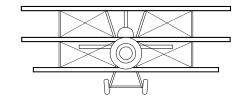
\includegraphics[width=0.33\textwidth]{01-EtudeAeronefs/img/ailes/Triplane.pdf}
  				\legende{Triplan}{wing:Triplane}	
			\end{figure}
	\end{multicols}
	
	\begin{figure}[H]
		\centering
		\begin{minipage}{.33\textwidth}
  			\centering
  			\includegraphics[width=0.9\textwidth]{01-EtudeAeronefs/img/DR400.jpg}
  			\legende{Monoplan moderne DR400}{img:DR400}	
		\end{minipage}%
		\begin{minipage}{.33\textwidth}
  			\centering
  			\includegraphics[width=0.9\textwidth]{05-Histoire/img/wrightFlyer.jpg}
  			\legende{Biplan Wright Flyer}{img:wrightFlyer}
		\end{minipage}
		\begin{minipage}{.33\textwidth}
  			\centering
	  		\includegraphics[width=0.9\textwidth]{05-Histoire/img/sopwithTriplane.jpg}
  			\legende{Triplan Sopwith Triplane}{img:sopwithTriplane}	
		\end{minipage}
	\end{figure}	
 		
 	\begin{multicols}{2}
 			\begin{figure}[H]
  				\centering
  				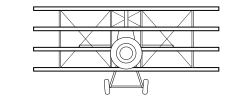
\includegraphics[width=0.33\textwidth]{01-EtudeAeronefs/img/ailes/Quadruplane.pdf}
  				\legende{Quadriplan}{wing:Quadruplane}	
			\end{figure}
			
			\begin{figure}[H]
  				\centering
  				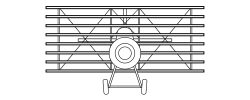
\includegraphics[width=0.33\textwidth]{01-EtudeAeronefs/img/ailes/Multiplane.pdf}
  				\legende{Multiplan}{wing:Multiplane}	
			\end{figure}
 	\end{multicols}
 
 \begin{multicols}{2}
	\begin{figure}[H]
  		\centering
  		\includegraphics[width=0.33\textwidth]{05-Histoire/img/bessonH5.jpg}
  		\legende{Quadriplan Besson H5}{img:bessonH5}	
	\end{figure}
	\begin{figure}[H]
  		\centering
  		\includegraphics[width=0.33\textwidth]{01-EtudeAeronefs/img/horatioPhillipsMultiplane.png}
  		\legende{Appareil doté de 20 plans (1904)}{img:horatioPhillipsMultiplane}	
	\end{figure}
 \end{multicols}
 
 	\subsubsection{Dièdre de l'aile}
 	\begin{multicols}{3}

 		\begin{figure}[H]
  		\centering
  		\includegraphics[width=0.33\textwidth]{01-EtudeAeronefs/img/ailes/Monoplane_dihedral.pdf}
  		\legende{Dièdre positif}{wing:Monoplane-dihedral}	
		\end{figure}

 \begin{figure}[H]
  		\centering
  		\includegraphics[width=0.33\textwidth]{01-EtudeAeronefs/img/ailes/Monoplane_mid.pdf}
  		\legende{Dièdre nul}{wing:Monoplane-mid}	
		\end{figure}

 \begin{figure}[H]
  		\centering
  		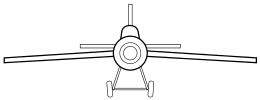
\includegraphics[width=0.33\textwidth]{01-EtudeAeronefs/img/ailes/Monoplane_anhedral.pdf}
  		\legende{Dièdre négatif}{wing:Monoplane-anhedral}	
		\end{figure}
 \end{multicols}
	
	\subsubsection{Forme d'ailes}
 
 \begin{figure}[H]
		\centering
		\begin{minipage}{.33\textwidth}
  			\centering
  			\includegraphics[width=1\textwidth]{01-EtudeAeronefs/img/ailes/Wing_constant.pdf}
  			\legende{Aile rectangulaire}{wing:Wing-constant}		
		\end{minipage}%
		\begin{minipage}{.33\textwidth}
  			\centering
  			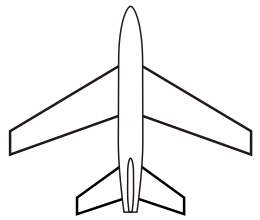
\includegraphics[width=1\textwidth]{01-EtudeAeronefs/img/ailes/Wing_swept.pdf}
  			\legende{Aile en flèche}{wing:Wing-swept}	
		\end{minipage}
		\begin{minipage}{.33\textwidth}
  			\centering
	  		\includegraphics[width=1\textwidth]{01-EtudeAeronefs/img/ailes/Wing_elliptical.pdf}
  			\legende{Aile elliptique}{wing:Wing-elliptical}	
		\end{minipage}
	\end{figure}	
 
 \begin{multicols}{3}
 \begin{figure}[H]
  		\centering
  		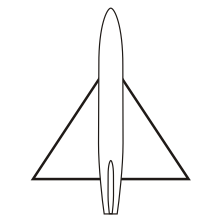
\includegraphics[width=0.33\textwidth]{01-EtudeAeronefs/img/ailes/Wing_tailless_delta.pdf}
  		\legende{Aile delta}{wing:Wing-tailless-delta}	
		\end{figure}
 \begin{figure}[H]
  		\centering
  		\includegraphics[width=0.33\textwidth]{01-EtudeAeronefs/img/ailes/Wing_ogival_delta.pdf}
  		\legende{Aile gothique}{wing:Wing-ogival-delta}	
		\end{figure}
 \begin{figure}[H]
  		\centering
  		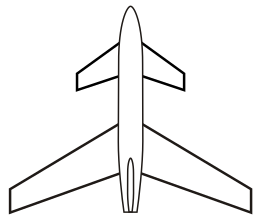
\includegraphics[width=0.33\textwidth]{01-EtudeAeronefs/img/ailes/Wing_canard.pdf}
  		\legende{Configuration canard}{wing:Wing-canard}	
		\end{figure}
 \end{multicols}
 
 \begin{multicols}{3}
 \begin{figure}[H]
  		\centering
  		\includegraphics[width=0.33\textwidth]{01-EtudeAeronefs/img/mirage2000.jpg}
  		\legende{Aile delta : chasseur}{img:mirage2000}	
		\end{figure}
 \begin{figure}[H]
  		\centering
  		\includegraphics[width=0.33\textwidth]{01-EtudeAeronefs/img/concorde.jpg}
  		\legende{Aile gothique : Concorde}{img:concorde}	
		\end{figure}

 \begin{figure}[H]
  		\centering
  		\includegraphics[width=0.33\textwidth]{01-EtudeAeronefs/img/rutanLongEz.jpg}
  		\legende{Canard : Long EZ}{img:rutanLongEz}	
		\end{figure}
 \end{multicols}
 
 	\subsubsection{L'aile}
 	Toutes les ailes \anglais{wing} des avions sont globalement conçues selon les mêmes principes.
 	
 	L'aile est construite autour d'un longeron, poutre maitresse qui permet de transférer la charge portée par l'aile au fuselage. Les nervures \anglais{rib} donnent à l'aile son profil. On fixe sur ces longerons la peau \anglais{skin}, qui constitue la partie visible de l'aile. Des raidisseurs permettent de donner une plus grande rigidité à l'aile.
 	\begin{figure}[H]
  		\centering
    		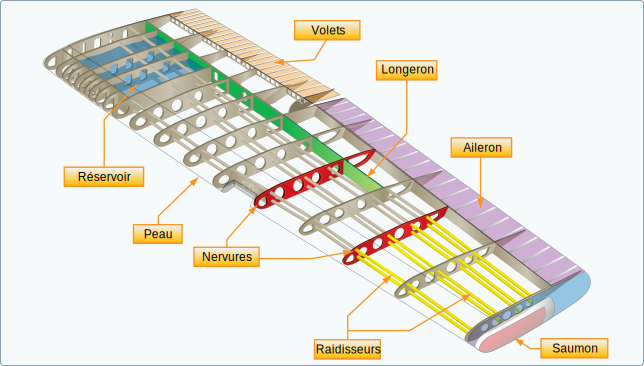
\includegraphics[width=0.75\textwidth]{01-EtudeAeronefs/img/schemaAile.pdf}
  		\legende{Les constituants d'une aile d'avion}{img:schemaAile}
	\end{figure}	
	
	En bout d'aile, le saumon \anglais{wing tip} accueil généralement des feux de navigation.
	
	Sur le bord de fuite et sur la partie extérieure de l'aile sont disposés les ailerons, qui permettent le contrôle en roulis de de l'avion. On dispose les volets \anglais{flap} sur le bord de fuite de l'aile du côté du fuselage.
	
	
	
	\subsubsection{Train d'atterrissage}

